\documentclass[a4paper,12pt]{book}
\usepackage[T1]{fontenc}
\usepackage[utf8]{inputenc}
\usepackage[francais]{babel}
\usepackage{lmodern}
\usepackage{multirow}
\usepackage{amsthm}
\usepackage{amsmath}
\usepackage{amssymb}
\usepackage{mathrsfs}
\usepackage{amsfonts}
\usepackage{latexsym}
\usepackage{graphicx}
\usepackage{moreverb}
\usepackage{url}
\usepackage{fancyhdr}
\usepackage{color}
\usepackage{wrapfig}
\usepackage{vector}
\usepackage{hyperref}
\usepackage{bardiag}
\usepackage{fancyhdr}

\newtheorem{solution}{Solution}[section]
\newtheorem{nom2}{Proposition}[section]
\newtheorem{exercice}{Exercice}[section]
\numberwithin{equation}{section}

\newcommand{\bra}[1]{\langle#1\vert}
\newcommand{\ket}[1]{\vert#1\rangle}
\renewcommand{\headrulewidth}{2pt}
\renewcommand{\footrulewidth}{2pt}

\usepackage[top=2.5cm, bottom=2.5cm, left=2.5cm, right=2.5cm]{geometry}
\usepackage{listings}
\usepackage[french]{minitoc-hyper}
\lhead{}
\chead{}
\rhead{}
% lignes horizontales (par défaut une au-dessus pas en-dessous)
%\renewcommand{\headrulewidth}{0pt}
%\renewcommand{\footrulewidth}{0.4pt}
% pied de page à gauche, au centre et à droite
\lfoot{}
\cfoot{Année académique 2012-2013}
\rfoot{\thepage}
\pagestyle{fancy}
\lstset{
language=Python,
basicstyle=\footnotesize,
numbers=left,
numberstyle=\footnotesize,
numbersep=7pt
}
\begin{document}

\chapter{Correction des exercices}
\label{chap:correct}

\bigskip

\section{Qubits et  états quantiques}
\subsection{Chat de Shr\"odinger}
Les états $\ket{\psi_1}$ et $\ket{\psi_2}$ sont donnes par :
\begin{equation}
\begin{array}{rcl}
\ket{\psi_1} &=& \dfrac{1}{\sqrt{2}}(\ket{m}+\ket{v})\\
\ket{\psi_2} &=& \dfrac{1}{2}(\sqrt{3}\ket{m}+\ket{v}).
\end{array}
\end{equation}

Pour les représenter sur la sphère de Bloch, on procède comme suit :
\begin{lstlisting}
#Chat de Shrodinger

from qutip import *
from pylab import *

#Definition des etats morts et vivants : ces etats representent les etats 0 et 1
mort = basis(2,0)
vivant = basis(2,1)
#Definition des etats Psi_1 et Psi_2
Psi_1 = (mort+vivant)/sqrt(2)
Psi_2 = (sqrt(3)*mort+vivant)/2

B=Bloch()
B.add_states([mort,vivant,Psi_1,Psi_2])
B.show()

\end{lstlisting}
\section{Mesure et opérateurs linéaires}
\subsection{Opérateurs dans QuTiP}
Le programme en QuTiP est le suivant
\begin{lstlisting}
# Operateurs dans QuTiP

from qutip import *
from pylab import *

ket0 = basis(2,0)
ket1 = basis(2,1)

#Definition des operateurs
X1 = [[0,1],[1,0]]
Y1 = [[0,-1j],[1j,0]]
Z1 = [[1,0],[0,-1]]
X1 = Qobj(X1)
Y1 = Qobj(Y1)
Z1 = Qobj(Z1)

X = sigmax()
Y = sigmay()
Z = sigmaz()

#Valeurs propres et vecteurs propres de X
[val1,val2],[vec1,vec2] = X.eigenstates()

Z*vec1
Z*vec2
# Z se comporte comme une porte NOT
# Definition de H
H = (X+Z)/sqrt(2)
[va1,va2],[ket1,ket2] = H.eigenstates()

H.isherm
HH = H*H
HH == qeye(2)
#H est hermitien et H*H = I, alors H est une matrice unitaire
# Calcul des projecteurs sur les etats propres de H
P1 = ket1*ket1.dag()
P2 = ket2*ket2.dag()

# Proprietes
P1.isherm
P1*P1 == P1

\end{lstlisting}


\subsection{Représentation matricielle}
En QuTiP, le programme est le suivant :
\begin{lstlisting}
#Representation matricielle

from qutip import *
from pylab import *

#Definition des etats des bases
Phi_1 = basis(3,0)
Phi_2 = basis(3,1)
Phi_3 = basis(3,2)

Psi_0 = Phi_1/sqrt(2)+1j*Phi_2/2+Phi_3/2
Psi_1 = (Phi_1+1j*Phi_3)/sqrt(3)

#Verification de la norme
Psi_0.norm()#Le resultat s'affiche en executant cette commande
Psi_1.norm()#Le resultat s'affiche en executant cette commande

#Calcul de P0 et P1
P0 = Psi_0*Psi_0.dag()
P1 = Psi_1*Psi_1.dag()

#Hermiticite
P0.isherm#Le resultat s'affiche en executant cette commande (True or False)
P1.isherm#Le resultat s'affiche en executant cette commande (True or False)

#Definition de Y
Y = sigmay()
Y.isherm

#Valeurs propres et vecteurs propres de Y
[Val1,Val2],[vec1,vec2] = Y.eigenstates()

#Projecteurs sur les etats propres
P_1 = vec1*vec1.dag()
P_2 = vec2*vec2.dag()

#Relation de fermeture et d'orthogonalite
P_1+P_2# On obtient la matrice Identite
P_1*P_2#On obtient la matrice nulle

\end{lstlisting}

\subsection{ECOC Avec QuTiP}
\begin{lstlisting}
# ECOC

from qutip import *
from pylab import *

#Definition des etats de base.
u1 = basis(3,0)
u2 = basis(3,1)
u3 = basis(3,2)

#Definition de l'operateur H.
H = [[2, -3*sqrt(2), 3*sqrt(2)],[-3*sqrt(2), -1, -3],[3*sqrt(2), -3, -1]]
H = Qobj(H) # Rendre H un objet Quantique

#Calcul des energies et vecteurs propres de H
[E1, E2,E3], [ketE1, ketE2, ketE3] = H.eigenstates()

#Resolution de l'equation de shrodinger
T = linspace(0,10,11) #Partitionner l'interval de temps
data = mesolve(H,u1,T,[],[H,H*H]) #Resolution de l'equation avec mesolve
Etat = data.states #Extraire les etats pour t dans [0,10]
MoyenH = data.expect[0] #Moyenne de H pour t dans [0,10]
MoyenHH = data.expect[1] # Moyenne de H*H pour t dans [0,10]
DeltaH = sqrt(MoyenHH[10]-MoyenH[10]**2)

#Projecteurs sur les etats propres de H
P1 = ketE1*ketE1.dag()
P2 = ketE2*ketE2.dag()
P3 = ketE3*ketE3.dag()

# K en fonction de P1, P2 et P3
K = P3+P2

# Valeurs propres et vecteurs propres de K
[k1,k2,k3] ,[ketk1,ketk2,ketk3] = K.eigenstates()
ketk1.dag()*H*ketk1
ketk2.dag()*H*ketk2
ketk3.dag()*H*ketk3

\end{lstlisting}

\section{Postulats et évolution}
\subsection{Moment magnétique du Deutéron}
Le programme en QuTiP est le suivant :
\begin{lstlisting}
# Moment magnetique du Deuteron

from qutip import *
from pylab import *

#Definition des etats de base
ketp = basis(3,0)
ket0 = basis(3,1)
ketm = basis(3,2)

#Hamiltonien du noyau
H = 1*ketp*ketp.dag()+0*ket0*ket0.dag()-1*ketm*ketm.dag()

#Matrice M=A
M = [[0,1,0],[1,0,1],[0,1,0]]
M = Qobj(M)
M = (1/sqrt(2))*M

#Calcul des valeurs propres et vecteurs propres
[val1,val2,val3],[vec1,vec2,vec3] = M.eigenstates()
#Projecteurs P1, P2,P3
P1 = vec1*vec1.dag()
P2 = vec2*vec2.dag()
P3 = vec3*vec3.dag()

#Valeur moyenne de M dans l'etat  Psi0
Psi0 = vec1
MoyM = expect(M,vec1)
MoyH = expect(H,Psi0)
MoyHH = expect(H*H,Psi0)
DeltaH = sqrt(MoyHH-MoyH**2)

#Valeur moyenne de M dans le temps
T = linspace(0,10,100)
data = mesolve(H,Psi0,T,[],[M,P1,P2,P3])
MoyMt = data.expect[0]
P1t = data.expect[1]
P2t = data.expect[2]
P3t = data.expect[3]

#Courbe de la valeur moyenne et des probabilités
plot(T,MoyMt,T,P1t,T,P2t,T,P3t)
xlabel('Temps')
title(("Moment magnetique du Deuteron"))
legend(("Moyenne de M","P1","P2","P3"))
show()

\end{lstlisting}

\begin{figure}[!h]
\begin{center}
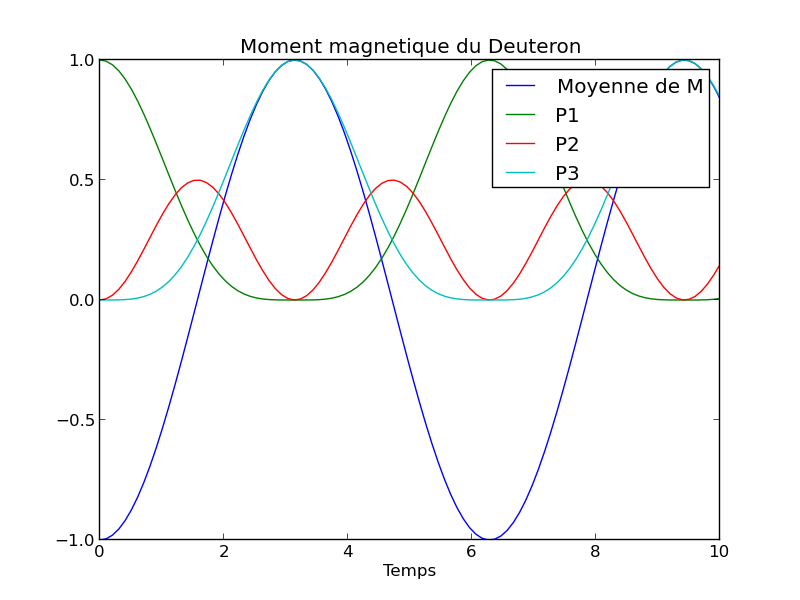
\includegraphics[height=8cm]{Images/NoyauDeuteron.png}
\end{center}
\end{figure}

\subsection{Evolution d'un état de spin 1/2}
Le programme est le suivant :
\begin{lstlisting}
from qutip import *
from pylab import *

#Hamiltonien H et ses etats propres
H = 0.25*sigmaz()
zp = basis(2,0)
zm = basis(2,1)
#Projecteurs sur les etats x+ et x-
xp = (zp+zm)/sqrt(2)
xm = (-zp+zm)/sqrt(2)
Pp = xp*xp.dag()
Pm = xm*xm.dag()
#Resolution de l' equation  de schrodinger
T = linspace(0,30,100)
data = mesolve(H, xp, T, [], [Pp,Pm,H,H*H])
P1 = data.expect[0]
P2 = data.expect[1]
MoyH = data.expect[2]
MoyHH = data.expect[3]
#Representation
plot(T, P1, T, P2)
xlabel('Temps $t$')
ylabel('Probabilite')
legend(("P+","P-"))
title(("Probabilite de transition"))
show()
#Calcul de la deviation standard
DeltaH = sqrt(MoyHH[99]-MoyH[99]**2)
\end{lstlisting}

\begin{figure}[!h]
\begin{center}
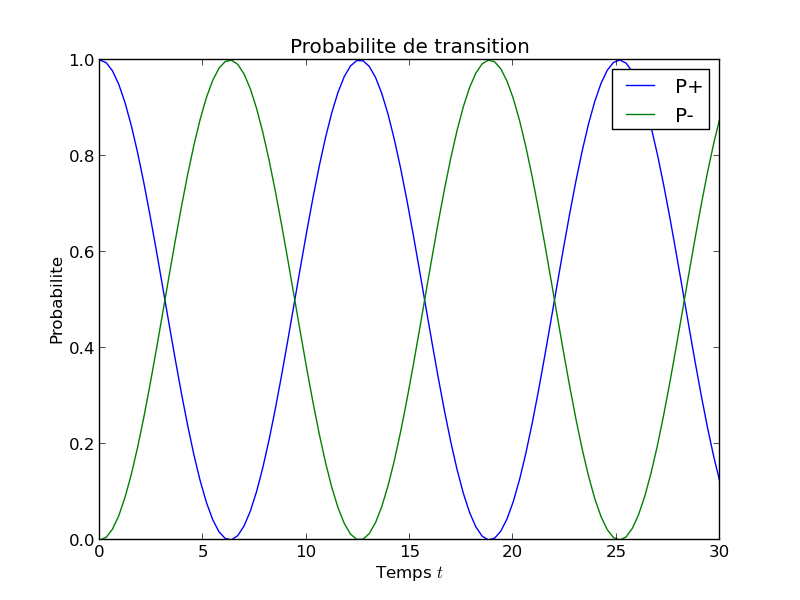
\includegraphics[height=8cm]{Images/Spin1_2.png}
\end{center}
\end{figure}

\section{Corrélations quantiques}
\subsection{Systèmes composites}
\begin{lstlisting}
#Systeme composite

from qutip import *
from pylab import *

#Definition des etats de base
ket0 = basis(2,0)
ket1 = basis(2,1)

ket00 = tensor(ket0,ket0)
ket01 = tensor(ket0,ket1)
ket10 = tensor(ket1,ket0)
ket11 = tensor(ket1,ket1)

#Definition des operateurs
X = sigmax()
Z = sigmaz()
I = qeye(2)
W = (X+Z)/sqrt(2)
H = tensor(X,Z)+tensor(W,I)

#Valeurs propres et vecteurs propres de H
[val1,val2,val3,val4],[ket1,ket2,ket3,ket4] = H.eigenstates()

Psi = H*ket00
Psi = Psi.unit()#unit() permet de normaliser un etat.
P = Psi.ptrace(0)
P*P == P

\end{lstlisting}

\subsection{Construction d'un état corrélé}
Le programme en QuTiP est le suivant :
\begin{lstlisting}
#Construction d'un etat correle

from qutip import *
from pylab import *

#Definition des etats de base

ket0 = basis(2,0)
ket1 = basis(2,1)

ket00 = tensor(ket0,ket0)
ket01 = tensor(ket0,ket1)
ket10 = tensor(ket1,ket0)
ket11 = tensor(ket1,ket1)

#Definition du hamiltonien
sigma12 = tensor(sigmax(),sigmax())+tensor(sigmay(),sigmay())+tensor(sigmaz(),sigmaz())
H = 0.5*sigma12

#Verification
I = tensor(qeye(2),qeye(2))
(I+sigma12)*ket00
(I+sigma12)*ket01
(I+sigma12)*ket10
(I+sigma12)*ket11

#Vecteurs propres et valeurs propres de H
[val1,val2,val3,val4],[ket1,ket2,ket3,ket4] = sigma12.eigenstates()

#
T = linspace(0,2*pi,80)
data = mesolve(H,ket10,T,[],[])
Psit = data.states
Psi = (ket10-1j*ket01)/sqrt(2)
fidelity(Psi*Psi.dag(),Psit[10]*Psit[10].dag())

\end{lstlisting}

\section{Calculs quantiques}
\subsection{Circuit intraportation avec QuTiP}
Une des programmes en QuTiP qui implémente le circuit intraportation est le suivant
\begin{lstlisting}
# Teleportation d'une paire EPR sans bruit

from qutip import *
from pylab import *

# Definitions des operateurs intervenants dans le programme
X = sigmax()
Z = sigmaz()
Y = sigmay()
W = (X+Z)/sqrt(2)
I = qeye(2)

CX_12 = tensor(ket0*ket0.dag(), I, I) + tensor(ket1*ket1.dag(), X, I)
W_1 = tensor(W, I, I)
CX_23 = tensor(I,ket0*ket0.dag(), I) + tensor(I,ket1*ket1.dag(), X)
CZ_13 = tensor(ket0*ket0.dag(), I, I) + tensor(ket1*ket1.dag(), I, Z)

# Definition de B
W_2 = tensor(W,I)
CX_23_1 = tensor(ket0*ket0.dag(), I) + tensor(ket1*ket1.dag(), X)
B = CX_23_1*W_2
U = CZ_13*CX_23*W_1*CX_12 # Operateur d'evolution du circuit de la teleportation

#Generer l'etat EPR
ket00 = tensor(ket0,ket0)
EPR = B*ket00

# Definition de l'etat d'entree
ket0 = basis(2,0)
ket1 = basis(2,1)
Psi = (ket0+ket1)/sqrt(2)
Psi_in = tensor(Psi, EPR)

# Calcul de l'etat de sortie (Psi_out et Rho_out)
Psi_out = U*Psi_in
Rho_Bob = Psi_out.ptrace(2)
Prob = Psi.dag()*Rho_Bob*Psi
\end{lstlisting}

\subsection{Téléportation d'une paire EPR}
Une façon d'écrire ce programme en QuTiP est le suivant
\begin{lstlisting}
# Teleportation d'une paire EPR

from qutip import *
from pylab import *

#Definitions des etats
ket0 = basis(2,0)
ket1 = basis(2,1)
Psi = (ket0+ket1)/sqrt(2)

# Definition des operateurs
X = sigmax()
Y = sigmay()
Z = sigmaz()
W = (X+Z)/sqrt(2)
I = qeye(2)

W_2 = tensor(I,W,I,I,I)
W_3 = tensor(W,I,I)
W_4 = tensor(I,I,I,W,I)
W_5 = tensor(I,I,I,I,W)

CX_12_1 = tensor(ket0*ket0.dag(), I) + tensor(ket1*ket1.dag(), X)
CX_12_2 = tensor(ket0*ket0.dag(), I, I) + tensor(ket1*ket1.dag(), X, I)
CX_13 = tensor(ket0*ket0.dag(), I, I) + tensor(ket1*ket1.dag(), I, X)
CX_14 = tensor(ket0*ket0.dag(),I,I,I,I) + tensor(ket1*ket1.dag(),I,I,X,I)
CX_23 = tensor(I,ket0*ket0.dag(),I,I,I) + tensor(I,ket1*ket1.dag(),X,I,I)
CX_24 = tensor(I,ket0*ket0.dag(),I,I,I) + tensor(I,ket1*ket1.dag(),I,X,I)
CX_34 = tensor(I,I,ket0*ket0.dag(),I,I) + tensor(I,I,ket1*ket1.dag(),X,I)
CX_35 = tensor(I,I,ket0*ket0.dag(),I,I) + tensor(I,I,ket1*ket1.dag(),I,X)
CX_54 = tensor(I,I,I,I,ket0*ket0.dag()) + tensor(I,I,I,X,ket1*ket1.dag())
CX_53 = tensor(I,I,I,I,ket0*ket0.dag()) + tensor(I,I,X,I,ket1*ket1.dag())
CX_51 = tensor(I,I,I,I,ket0*ket0.dag()) + tensor(X,I,I,I,ket1*ket1.dag())

#Definitions des etats
ket0 = basis(2,0)
ket1 = basis(2,1)
Psi = (ket0+ket1)/sqrt(2)
# Generation des etats EPR et GHZ
EPR = CX_12_1*tensor(Psi, ket1)
GHZ = CX_13*CX_12_2*W_3*tensor(ket0, ket0, ket0)
#etat d'entree
Psi_in = tensor(EPR,GHZ)

# Operateur d'evolution du circuit
U = CX_51*W_5*CX_14*CX_54*CX_35*W_4*CX_24*W_4*CX_34*W_2*CX_23*W_2

# Calcul de l'etat de sortie du circuit
Psi_out = U*Psi_in
Rho_5 = Psi_out.ptrace(4)

# Comparaison : calcul de la probabilite
Proba = Psi.dag()*Rho_5*Psi
\end{lstlisting}
\end{document}
